\documentclass[a4paper,11pt, notitlepage]{article}
\usepackage{xspace} % define commands with auto-spacing command \xspace
\usepackage[absolute]{textpos}
\usepackage[english]{babel}
\usepackage[utf8]{inputenc} % unicode encoding
\usepackage{titlesec}
\usepackage[left=3.5cm, right=3.5cm]{geometry}
\usepackage{enumerate}
\usepackage{setspace}
\usepackage{graphicx} % support for \includegraphics{}
\usepackage[section]{placeins}
\usepackage{todonotes}
\usepackage{float}
\usepackage[plainpages=false]{hyperref}
\usepackage{fancyvrb}
\usepackage{eurosym}
\usepackage{listings}
\usepackage{amsmath}

\newcommand{\IaaS}{IaaS\xspace}
\newcommand{\adal}{ADAL\xspace}
\newcommand{\PaaS}{PaaS\xspace}
\newcommand{\SaaS}{SaaS\xspace}
\newcommand{\aad}{\azure \emph{Active Directory}\xspace}
\newcommand{\wsfed}{WS-Fed\xspace}
\newcommand{\sso}{{Single Sign-on}\xspace}
\newcommand{\BetoSys}{\emph{BetoSys}\xspace}
\newcommand{\Idaas}{IdaaS\xspace}
\newcommand{\azure}{\emph{Azure}\xspace}
\newcommand{\serviceprov}{Service Provider\xspace}
\newcommand{\idp}{Identity Provider\xspace}
\newcommand{\public}{\emph{Public Cloud}\xspace}
\newcommand{\private}{\emph{Private Cloud}\xspace}
\newcommand{\community}{\emph{Community Cloud}\xspace}
\newcommand{\hybrid}{\emph{Hybrid Cloud}\xspace}
\newcommand{\code}[1]{\texttt{#1}} %texttt oder textsc
\newcommand{\expectedres}{\textbf{Erwartetes Ergebnis}}
\newcommand{\cmark}{\textcolor{green}{\ding{51}}}
\newcommand{\xmark}{\textcolor{red}{\ding{55}}}
\newcommand{\enq}[1]{\grqq{}#1\grqq{}}

\lstset
{ %Formatting for code in appendix,
	basicstyle=\footnotesize,
	numbers=left,
	stepnumber=1,
	showstringspaces=false,
	tabsize=1,
	breaklines=true,
	breakatwhitespace=false,
	literate={ö}{{\"o}}1
	{ä}{{\"a}}1
	{ü}{{\"u}}1
	{Ö}{{\"O}}1
	{Ä}{{\"A}}1
	{Ü}{{\"U}}1
}


%\newcommand{\code}[1]{\texttt{#1}}

\onehalfspacing
\setlength{\parindent}{0pt}
\titleformat{\chapter}[display]{\normalfont\huge\bfseries\filcenter}{\chaptertitlename\ \thechapter}{20pt}{\Huge}
\titlespacing*{\chapter}{0pt}{-50pt}{40pt}




%%%%%%%%%% Your Document starts here %%%%%%%%%%
\begin{document}
	
	\fontfamily{phv}
	\selectfont
	% fill in these additional information

% Name of the institute your work is submitted to 
\newcommand{\institute}{University of Wisconsin-Milwaukee}
% Name of the department your work is submitted to 
\newcommand{\instituteDepartment}{Department of Mathematics}
% Kind of work this is e.g. Bachelor of Science Thesis
\newcommand{\workSpecification}{Numerical Analysis}
% Title of your work
\newcommand{\workTitle}{Comparing different Methods of Interpolation}


%Layoutaenderung dank Corporate Design
%\newgeometry{top=4.2cm, bottom=1.3cm, left=2cm, right=2cm}

\begin{titlepage}	
	\begin{center}
		% Upper part of the page
		
%		\begin{textblock*}{1mm}(25mm,10mm)
%			\includegraphics[height=30mm]{./images/logo-fh.png}
%		\end{textblock*}
		~\\
		\vspace{1cm}
		\fontsize{18pt}{16}\selectfont
		\institute\\
		\Large \instituteDepartment\\
		\vspace*{5cm}
		\textsc{\Large \workSpecification} \bigskip
				
		% Title
		\hrule \par\bigskip
		\textbf\workTitle

		\par\bigskip
		\hrule \par\bigskip
		% Author and supervisor
		\vspace{2cm}
		
		\large{\setstretch{1.5}{
				Jan Kretschmann
		}}
	
	

		%\vfill \vfill\vfill 
		%	\noindent\rule{0.4\textwidth}{0.5pt} \hfill \noindent\rule{0.4\textwidth}{0.5pt}\\ 
		%	(Unterschrift Betreuer) \hfill (Unterschrift Auszubildender)
			
		

		% Bottom of the page
		
	\end{center}
	
\end{titlepage}

%Layout CD aus
%\restoregeometry

	\begin{onehalfspace}
		
\section{Abstract} 
\label{sec:Abstract}	
In this work, different methods of interpolation are examined regarding their stability, accuracy, implementation and their behavior on specific problem settings. For this examination, a small dataset as well as a number of pre-defined functions were used. To compare the error, cross validation was applied to the small dataset, whereas the approximated results were directly compared to the actual results of the pre-defined functions.

It is found that the interpolation methods that yield algebraic approximation polynomials (such as Lagrange Interpolation and the related methods Newton's Divided Differences and Neville's Method) are similarly accurate for small to medium sized data sets, but accumulate a huge error as the size of the dataset increases. This phenomena is called numerical instability. 

In contrast, it can be seen that interpolation methods which yield non-algebraic approximation polynomials, such as the Natural Cubic Spline Interpolation, are numerically stable, and only increase in accuracy with increasing number of given data points.
\newpage

\section{Related Work}
\label{sec:Related Work}
Comparing methods of interpolation is not a new area of interest, and numerous papers have been published that are set to compare different methods of interpolation in certain categories.\\

For instance, the work \enq{Comparison of spline and Lagrangian interpolation} \cite{mcnamee1986comparison}, published in the \emph{Journal of Computational and Applied Mathematics} in 1986, compares the errors in Lagrange Interpolation polynomials to those in Cubic Spline Interpolation Polynomials. The author uses Neville's Method to compute Lagrange Polynomials, and compares those to Cubic Spline Polynomials on several functions. 

He generates a dataset by computing function values in different step sizes starting from an initial point. It is found in this paper, that with large step-sizes, Lagrange Polynomials achieve an approximation that is much closer to the result than Cubic Spline Polynomials, but what is especially interesting is that it is also stated, that with small step sizes, both methods are \enq{about equally good}.

This is an interesting result, because in this work, it will be found that for increasing number of data points, Lagrange Polynomials will accumulate a huge error due to their instability. However, the reason for these conflicting results lies in the different application of Lagrange polynomials: even though the author uses step sizes as low as 0.01, only 3 data points are used for every evaluation, which is not enough to see the numerical instability of the Lagrange method.\\

%Another paper concerning a similar topic was published similarly long ago in 1982: \enq{A comparison of algorithms for polynomial interpolations}, by Allan Macleod \cite{macleod1982comparison}. 

%The author compares eight different methods of computing interpolation polynomials, including the Lagrangian form and Neville's Method, which are both relevant for this work. However, the paper mainly focuses on the computational efficiency, as well as the stability regarding rounding errors accumulated by the methods.

%It is found that a modified version of Neville's method is among the most accurate and efficient in computing interpolation polynomials. However, instead of trying to find a function that interpolates the entire dataset, the author only considers a subset of the dataset every time he computes an approximation. For example, given a point $x$, which is not in the dataset, only the $N$ (for some positive integer $N$) points from the dataset that are closest to $x$ are taken to compute an interpolation polynomial, which is then used to approximate $x$.\\

\cite{mcnamee1986comparison} is examining the interpolation methods from a different viewpoint, especially compared to this work. It is to be remembered, that in the time the paper was published (the 1980s), computational power was much more expensive and way more restricted than nowadays. An example of a more recent work was published by Berrut in 2004: \enq{Barycentric lagrange interpolation} \cite{berrut2004barycentric}, which introduces a stable version of the Lagrange Interpolation Method. In the comparisons to the so called \emph{Barycentric} Lagrange Interpolation, the authors also find the error of the standard Lagrange approach to explode as the dataset increases in size, which is more similar to the focus of this work.

\section{Description of Methods}
\label{sec:Description}

\subsection{Piecewise Linear Interpolation}
\label{subsec:LinearInt}
Linear Interpolation describes the Method of taking two points from a dataset, and fitting a straight line through those points. This becomes increasingly inaccurate, the larger the distance between those two points is. Furthermore, if there are more than two points in the given dataset, it is impossible for a straight line to fit all the data points, unless they were taken from a straight line to begin with. \\
For these reasons, with larger datasets, the option that is mostly opted for is what is called \emph{Piecewise Linear Interpolation}. With Piecewise Linear Interpolation, one straight line is fitted between every two consecutive points of the dataset. This results in a continuous curve, with a non-continuous derivative.\\

For example, Figure \ref{fig:pw-linear-example} depicts the piecewise linear function that interpolates the points 


$$X = \{(0, 0), (3, 3), (5, 2), (6, 0)\}$$
The function is defined as:
\[
	P(x)=\begin{cases}
		x & 0 \leq x \leq 3 \\
		-0.5x+4.5 & 3 \leq x \leq 5 \\
		-2x+12 & 5 \leq x \leq 6
	\end{cases}
\]

\begin{figure}[H]
	\centering
	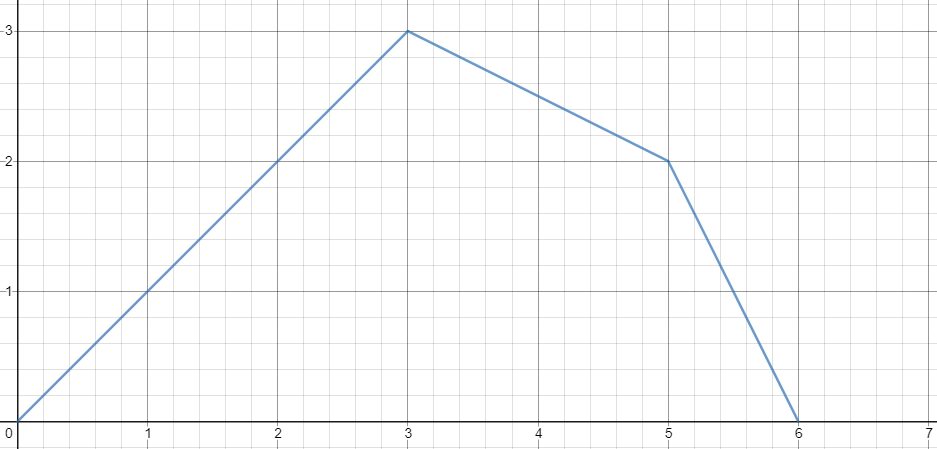
\includegraphics[width=\textwidth]{./images/pw-linear-example.png}
	\caption{Example of a Piecewise Linear Function.}
	\label{fig:pw-linear-example}
\end{figure}

\subsection{Lagrange Interpolation}
\label{subsec:Lagrange}
A standard Lagrange interpolating polynomial passes through every point in a given dataset while at the same time remaining algebraic: if there are $n+1$ data points, the polynomial will be of degree $n$ \cite{burden1985numerical}. \\
Lagrange polynomials are constructed as follows: 
$$P(x)=\sum_{k=0}^{n}f(x_k)L_{n, k}(x)$$
with $L{n, k}(x)=\prod_{i=0, i\neq k}^{n}\frac{x-x_i}{x_k - x_i}$. It can be seen, that the Lagrange polynomial is constructed to fit every point in the dataset: for every $i \neq k$, $L_{n, k}(x_i)$ will be equal to 0, and $L_{n, k}(x_k)=1$, so that $P(x_k)=f(x_k)$ holds for every $k$ \cite{burden1985numerical}.

In Figure \ref{fig:lag-example}, an example of a Lagrange interpolating polynomial can be seen. It was generated through the points 
$$X = {(-1, 1), (0, 0), (1, 1)}$$
so the resulting polynomial was computed to be
$$P(x) = \frac{(x-1)(x-0)}{(-1-1)(-1-0)} + \frac{(x+1)(x-0)}{(1+1)(1-0)}=x^2$$
which fits all the points in $X$.

\begin{figure}[H]
	\centering
	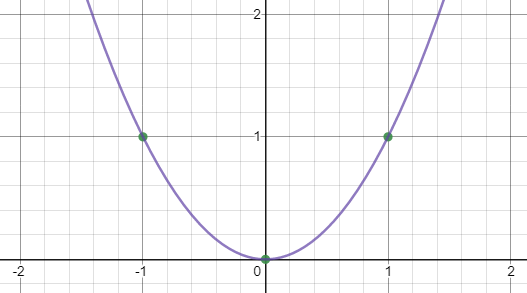
\includegraphics[width=\textwidth]{./images/lag-example.png}
	\caption{Example of a Lagrange interpolating polynomial.}
	\label{fig:lag-example}
\end{figure}

This form of Lagrange Interpolation brings two problems. Firstly, due to the Lagrange polynomial being algebraic, it loses numerical stability. This means, it becomes increasingly imprecise and accumulates a huge error, when $n$ gets large.
Secondly, Lagrange polynomials have an error term of $\frac{f^{(n+1)(\xi(x))}}{(n+1)!}\prod_{i=0}^{n}(x-x_i)$, which is generally not known when the function $f$ is not known, like in the example given above. Therefore, it makes sense to assume that the most precise approximation is the one that was made using every value of the dataset, even though sometimes that might be false (compare Illustration, Ch. 3.2 \cite{burden1985numerical}). Generating more than one Lagrange interpolation polynomial is not very efficient, because it contains the same amount of work every time.

\subsubsection{Neville's Method}
\label{subsubsec:Neville}
Neville's Method tries to address the problem of generating more than one Lagrange polynomial efficiently, by constructing them in an iterative way \cite{burden1985numerical}. It gives an algorithm, that generates a higher order Lagrange polynomial using already generated, lower order Lagrange Polynomials.\\
The algorithm for Neville's method, implemented in Python, can be seen in Figure \ref{fig:longbottom}\footnote{It can also be found in the separately uploaded Jupyter Notebook, in case the font is to small.}.

\begin{figure}[H]
	\centering
	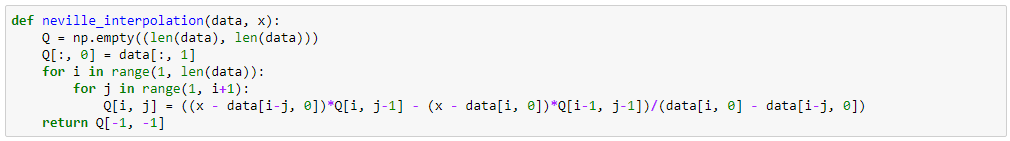
\includegraphics[width=\textwidth]{./images/neville-alg.png}
	\caption{Python Implementation of Neville's Algorithm.}
	\label{fig:longbottom}
\end{figure}


\subsubsection{Newton's Divided Differences}
\label{subsubsec:Newton}
Using Newton's Divided Differences is another way to address the issues the standard Lagrange Interpolation brings: instead of iteratively generating polynomials of higher order, Newton's Method successively generates polynomials of degree $<n$, that sum up to the Lagrange polynomial or order $n$. \\
The evaluation of an interpolation polynomial constructed with Newton's Divided Differences can be computed reasonably fast, using an algorithm called \emph{Horner's Scheme}.\\
The implementation of this algorithm can be found in Figure \ref{fig:newton}\footnote{It can also be found in the mentioned Jupyter Notebook.}.

\begin{figure}[H]
	\centering
	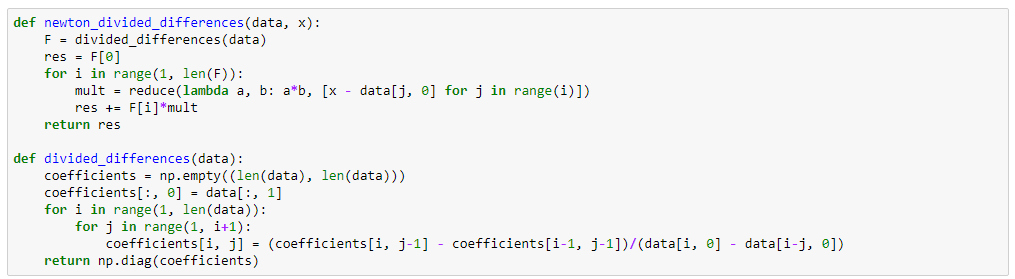
\includegraphics[width=\textwidth]{./images/newton-alg.png}
	\caption{Python Implementation of Newton's Divided Differences Algorithm.}
	\label{fig:newton}
\end{figure}

\subsubsection{First Comparison}
\label{subsubsec:fstcmp}
The first three interpolation methods described all result in the same Lagrange polynomial, they merely describe different algorithms to compute it. \\
The effect of computing the Lagrange polynomial using Newton's or Neville's Algorithms can already be seen in small examples: trying to interpolate the function $f(x)=x^4$ on the interval $[-10, 10]$ with 200 equally spaced data points, the Lagrange polynomial can only be computed\footnote{Machine: Windows PC, 16GB DDR3 RAM, Intel i7 3770k CPU, Python running on a single Thread. Implementation of Lagrange method can be found in Jupyter Notebook.} using Neville's or Newton's Algorithm, see Figure \ref{fig:nev-new-x4}.

 \begin{figure}
 	\centering
 	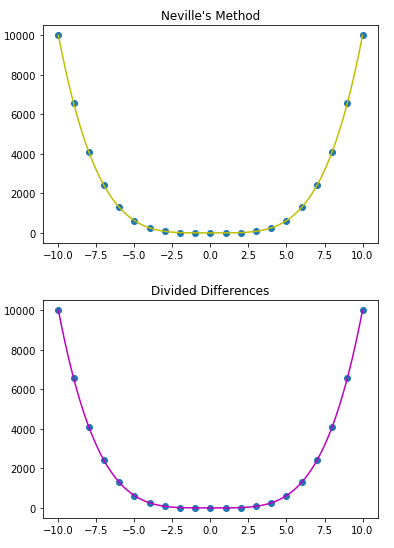
\includegraphics[width=\textwidth]{./images/nevnewx4.png}
 	\caption{Interpolating $f(x)=x^4$ using Neville's Method and Newton's Divided Differences.}
 	\label{fig:nev-new-x4}
 \end{figure}

However, when trying to interpolate the same dataset using the standard Lagrange method, the machine prints out an error, and the resulting polynomial can be seen in Figure \ref{fig:lag-x4}\footnote{Attention: the data points look like they are on a straight line here rather than on $f(x)=x^4$, this is due to the scaling of the Y-Axis.}. The error message can be seen in Figure \ref{fig:lag-x4-error}.

 \begin{figure}[H]
	\centering
	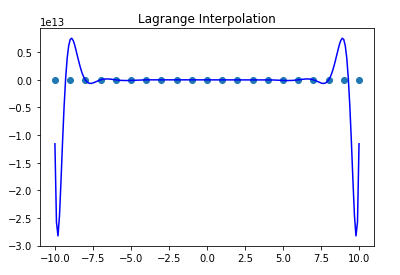
\includegraphics[width=\textwidth]{./images/lag-x4.png}
	\caption{Interpolating $f(x)=x^4$ using the standard Lagrange method.} 
	\label{fig:lag-x4}
\end{figure}

 \begin{figure}[H]
	\centering
	
\includegraphics[width=\textwidth]{./images/lag-x4-error.png}
	\caption{Error message when trying to interpolate $f(x)=x^4$ using the standard Lagrange method.}
	\label{fig:lag-x4-error}
\end{figure}


\subsection{Natural Cubic Spline Interpolation}
\label{subsec:cs}
In contrast to the previously described methods of interpolation, the Cubic Spline approach results in a piecewise-defined function, and not in a single polynomial \cite{burden1985numerical}. In theory, the advantage of this approach lies in its stability for large datasets: trying to compute a Lagrange polynomial for a large number of data points results in a high degree polynomial. Those, however, tend to \enq{oscillate erratically} \cite{burden1985numerical}. The Cubic Spline approach only contains functions of degree 3, and results in one cubic function between every interval of two consecutive points. This eliminates the instability that causes oscillation and results in higher accuracy, the more data points are given.\\
Cubic Spline polynomials are constructed as 
$$S_j(x)=a_j + b_j(x-x_j)+c_j(x-x_j)^2 +d_j(x-x_j)^3$$
with parameters, $a_j, b_j, c_j, d_j$ for $j=0,...,n-1$. A cubic spline satisfies the boundary conditions:
\begin{enumerate}
	\item $S_j(x)$ is cubic and defined on $[x_j, x_{j+1}]$
	\item $S_j(x_j)=f(x_j)$ and $S_j(x_{j+1})=f(x_{j+1})$
	\item $S'_{j+1}(x_{j+1})=S'_j(x_{j+1})$
	\item $S''_{j+1}=S''_j(x_{j+1})$
\end{enumerate}

Natural cubic splines also satisfy the boundary condition $S''(x_0)=S''(x_n)=0$ \cite{burden1985numerical}.\\
The construction of the natural cubic spline shows that $S_j(x_j)=a_j=f(x_j)$, and the remaining parameters can be solved by the equation system $Ax=b$, with
$$A=\begin{pmatrix}
	1 & 0 & 0 & ...& & 0 \\
	h_0 & 2(h_0 + h_1) & h_1 & ... & & 0 \\
	0 & h_1 & 2(h_1 + h_2) & h_2 & ... & 0\\
	... & ... & ... & ... & ... & 0\\
	& ... &  & h_{n-2} & 2(h_{n-2} + h_{n-1}) & h_{n-1} \\
	0 & ... & & & & 1   
\end{pmatrix}$$
with $h_i = x_{i+1} - x_i$,
$$x=\begin{pmatrix}
	c_0 \\
	...\\
	c_n
\end{pmatrix}$$
and $d_j = \frac{c_{j+1} - c_j}{3h_j}$, using the given boundary conditions \cite{burden1985numerical}. \\
It can be seen above, that the construction of a cubic spline is more complex than that of a Lagrange polynomial, especially using Neville's or Newton's Method. An implementation to find a Natural Cubic Spline polynomial according to Algorithm 3.4 in \cite{burden1985numerical} can be found in the uploaded Jupyter Notebook.


\section{Comparison of Interpolation Methods and Main Result}
\label{sec:Comparison}

\subsection{Comparison on dataset}
\label{subsec:compset}
Each method was implemented in Python according to the algorithms given in \cite{burden1985numerical}. Then, to compare the different approaches, they were used to interpolate a dataset from p. 141 of \cite{burden1985numerical}, which can be found in Table \ref{tab:databook}.

\begin{table}[H]
	\centering
	\begin{tabular}{|l|l|l|l|l|l|l|l|l|}
		\hline
		x & 0  & 3  & 5  & 8  & 13 \\ \hline
		y & 75 & 77 & 80 & 74 & 72 \\ \hline
	\end{tabular}
	\caption{dataset used for the comparison of interpolation methods.}
	\label{tab:databook}
\end{table}

The graphs of the different interpolation polynomials can be seen in Figures 



\begin{figure}[H]
	\centering
	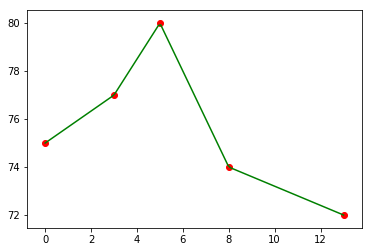
\includegraphics[]{./images/pw-dataset.png}
	\caption{Piecewise Linear Interpolation of the given dataset.}
	\label{fig:pw-dataset}
\end{figure}

\begin{figure}[H]
	\centering
	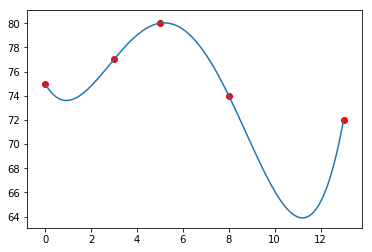
\includegraphics[]{./images/lag-dataset.png}
	\caption{Lagrange Interpolation Polynomial of the given dataset.}
	\label{fig:lag-dataset}
\end{figure}
As expected, the graphs produced by Neville's Method, Newton's Divided Differences and the standard Lagrange polynomial produce the same output, so only one is shown in Figure \ref{fig:lag-dataset}.

\begin{figure}[H]
	\centering
	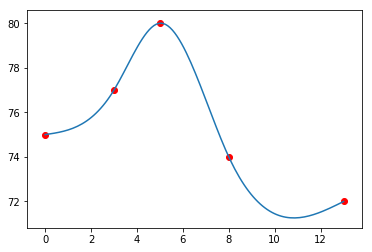
\includegraphics[]{./images/cs-dataset.png}
	\caption{Cubic Spline Interpolation Polynomial of the given dataset.}
	\label{fig:cs-dataset}
\end{figure}

When interpolating this small dataset, the oscillation that occurs in algebraic polynomials with high degrees can already be seen in the Lagrange polynomial. On the interval $[10, 12]$, the polynomial reaches $y$ values as low as 64, which is not indicated to happen anywhere in the dataset. The Cubic Spline polynomial, however, has a minimum that is barely below $y=72$. The difference is clearly visible in Figure \ref{fig:cs-lag-dataset}, where the Lagrange Polynomial is shown in black and the Cubic Spline in blue.

\begin{figure}[H]
	\centering
	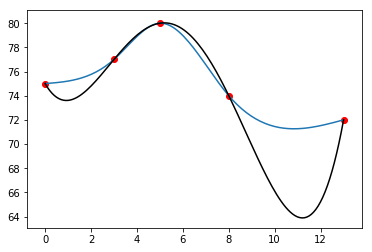
\includegraphics[]{./images/cs-lag-dataset.png}
	\caption{Comparison of Cubic Spline and Lagrange Polynomial.}
	\label{fig:cs-lag-dataset}
\end{figure}

To evaluate the accuracy of the different interpolation techniques on this dataset, where the exact function $f$ is unknown, cross validation was used. This is a common approach in machine learning, and it means the dataset was partitioned in \enq{training}(in this case interpolating) data and testing data. The algorithm is then evaluated on the training data, and knowing the result of the testing data, it can then be used to measure the accuracy of the interpolation polynomial. \\

In this particular case, let the dataset be $D=\{p_1, p_2, p_3, p_4, p_5\}$, with $p_i=(x_i, y_i)$. In each step, one $p_j$ was taken from the dataset to be the testing point. The interpolation methods were used with $D^*=\{p_i|i\neq j\}$, to compute an interpolation polynomial $P(x)$. At the end of each step, the difference $|P(x_j) - y_j|$ was accounted for as error. \\
Using this method, the errors for the examined methods can be found in Table \ref{tab:cv-errors}. \\
Obviously, all the Lagrange polynomials generate the same absolute error. As expected, the Natural Cubic Spline has less absolute error than the Lagrange polynomials. Surprisingly, the lowest error in this case was accumulated by the piecewise linear interpolation, which seems to be the most accurate for the given dataset.

\begin{table}[H]
	\centering
	\begin{tabular}{|l|l|l|l|l|l|}
		\hline
		Method & PW-Linear & Lagrange & Neville & Newton & Spline \\ \hline
		Error  & 8.2       & 17.39    & 17.39   & 17.39  & 12.98  \\ \hline
	\end{tabular}
	\caption{Comparison of errors of the different Interpolation Methods.}
	\label{tab:cv-errors}
\end{table}


\subsection{Comparison on Predefined Function}
\label{subsec:cmppre}
To get a more accurate comparison of the accuracy of the interpolating methods, they were also used to interpolate the functions
\begin{itemize}
	\item $f_1(x)=e^x$
	\item $f_2(x)=\sin(x)$
	\item $f_3(x)=x$
	\item $f_4(x)=x^4$
\end{itemize}
For this test, the respective functions were first evaluated on 40 equally spaced points on the interval $[0, 6]$, in order to get a dataset for the interpolation. All the methods were used to generate interpolation polynomials $P_j$ from this dataset. Then, to measure the accuracy, the points $\{(0.5+i, f_j(0.5+i))|i=0,...,5, j=1,...,4\}$ were computed. The absolute error for the function used in this work is summed up as follows:
$$e_j=\sum_{i=0}^{5}|f_j(0.5+i) - P_j(0.5+i)|$$

The resulting absolute errors can be found in Table \ref{tab:acc-pred}. It can be seen, that the Lagrange polynomials seem to be about as accurate as the spline polynomials under these circumstances, as also found in \cite{mcnamee1986comparison}, see Section \ref{sec:Related Work}. \\
The differences between the different ways to compute Lagrange polynomials can be attributed to machine imprecision: \emph{NumPy} was used in programming the methods, and as seen in the Jupyter Notebook at the very beginning, the default datatype in \emph{NumPy} has a precision of roughly $1.19 \times 10^{-7}$.

\begin{table}[H]
	\centering
	\begin{tabular}{|l|l|l|l|l|l|}
		\hline
		& PW-Linear & Lagrange               & Neville                & Newton                  & Spline                  \\ \hline
		$e^x$               & 0.25024   & $1.335 \times 10^{-6}$ & $3.853 \times 10^{-8}$ & $2.357 \times 10^{-7}$ & 0.00018                 \\ \hline
		$\sin(x)$               & 0.00357   & $2.818 \times 10^{-8}$ & $4.021 \times 10^{-9}$ & $7.414 \times 10^{-9}$  & $7.008 \times 10^{-7}$ \\ \hline
		$x$                    & 0         & $9.853 \times 10^{-8}$ & $3.409 \times 10^{-8}$ & 0                       & 0                       \\ \hline
		$x^4$ & 0.68810   & $5.014 \times 10^{-6}$ & $1.910 \times 10^{-7}$ & $3.640 \times 10^{-7}$  & 0.00019                 \\ \hline
	\end{tabular}
	\caption{Main Results regarding Accuracy: Accuracy of Interpolation Methods on predefined Functions.}
	\label{tab:acc-pred}
\end{table}


\subsection{Main Result regarding Stability}
\label{subsec:stab}
One thing, that was mentioned in \ref{subsec:cs}, is that the Cubic Spline Interpolation is stable, while Lagrange polynomials, due to them being algebraic, generally are not. \\
And this can be seen when comparing the development of the error of the Lagrange polynomial to that of a Cubic Spline polynomial, as the number of data points increases: working still on the interval $[0,6]$, the amount of error was examined for everything between 5 and 500 data points. \\
First we can see, the Piecewise Linear Interpolation polynomial, which gets more and more accurate the larger the dataset gets (see Figure \ref{fig:cs-bign}), and is almost equal to 0 once the polynomial is evaluated at all 200 nodes.

\begin{figure}[H]
	\centering
	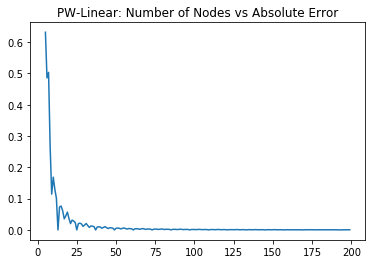
\includegraphics[]{./images/pw-lin-bign.png}
	\caption{Piecewise Linear Interpolation Polynomial: Error vs Number of Data Points.}
	\label{fig:pw-lin-bign}
\end{figure}

We see very similar behavior for the Cubic Spline Polynomial, compare Figure \ref{fig:cs-bign}, it approaches 0 the larger the dataset gets.

\begin{figure}[H]
	\centering
	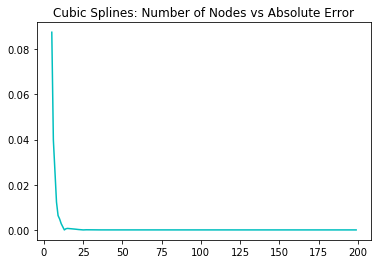
\includegraphics[]{./images/cs-bign.png}
	\caption{Cubic Spline Polynomial: Error vs Number of Data Points.}
	\label{fig:cs-bign}
\end{figure}

However, for the Lagrange polynomials, it is a different story: their numerical instability is clearly visible as the number of data points gets bigger: every method of computing Lagrange polynomials has an exploding error when the dataset gets too large\footnote{Notice, the Y-Axes are scaled in $10^{46}$, $10^{44}$ and $10^{45}$, so the error is not 0 at the beginning.}. This is explained by the oscillating of polynomials of high degree, as mentioned earlier and in \cite{burden1985numerical}. The error figures for all Lagrange polynomials can be seen in Figure \ref{fig:lag-all-bign}. Again, slight differences between the different methods are accounted for by machine imprecision.

\begin{figure}[H]
	\centering
	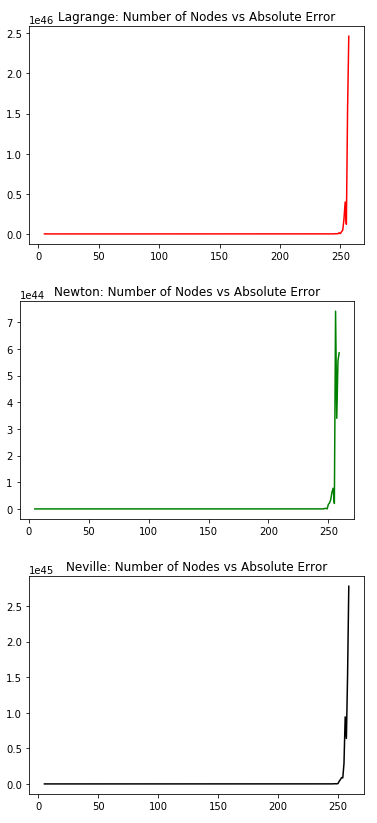
\includegraphics[]{./images/lag-all-bign.png}
	\caption{Piecewise Linear Interpolation Polynomial: Error vs Number of Data Points.}
	\label{fig:lag-all-bign}
\end{figure}


\section{Conclusion}
\label{sec:Conclusion}
From the data gathered, there is no one method that is always the right one. It was seen, that Lagrange interpolation is similarly accurate to Natural Cubic Spline Interpolation on smaller datasets. \\
As the datasets get larger, however, the numerical instability of the Lagrange method is visible, it accumulates a huge error due to oscillation of high degree polynomials, while the spline and piecewise-linear interpolation polynomials got more accurate. This is a striking difference between those polynomials examined that are algebraic, and those that are not. \\
On the ground of what was observed, it is impossible to make a recommendation for what interpolation method to use on small to medium sized datasets. However, as the number of data points gets larger (and the points are closer together), the non-algebraic interpolation methods seem to be superior. 


\newpage


\bibliography{literature}
\bibliographystyle{alpha}

\end{onehalfspace}
\end{document}